\section*{Описание методики COCOMO}
Модель COCOMO (COnstructive COst MOdel) разработана Барри Боэмом
(директор USC Center for Software Engineering). Это одна из основных методик,
которые применяются для оценки стоимости ПО. Среди других методик она
выгодно отличается простотой расчетов.

\begin{figure}[!h]
	\centering
	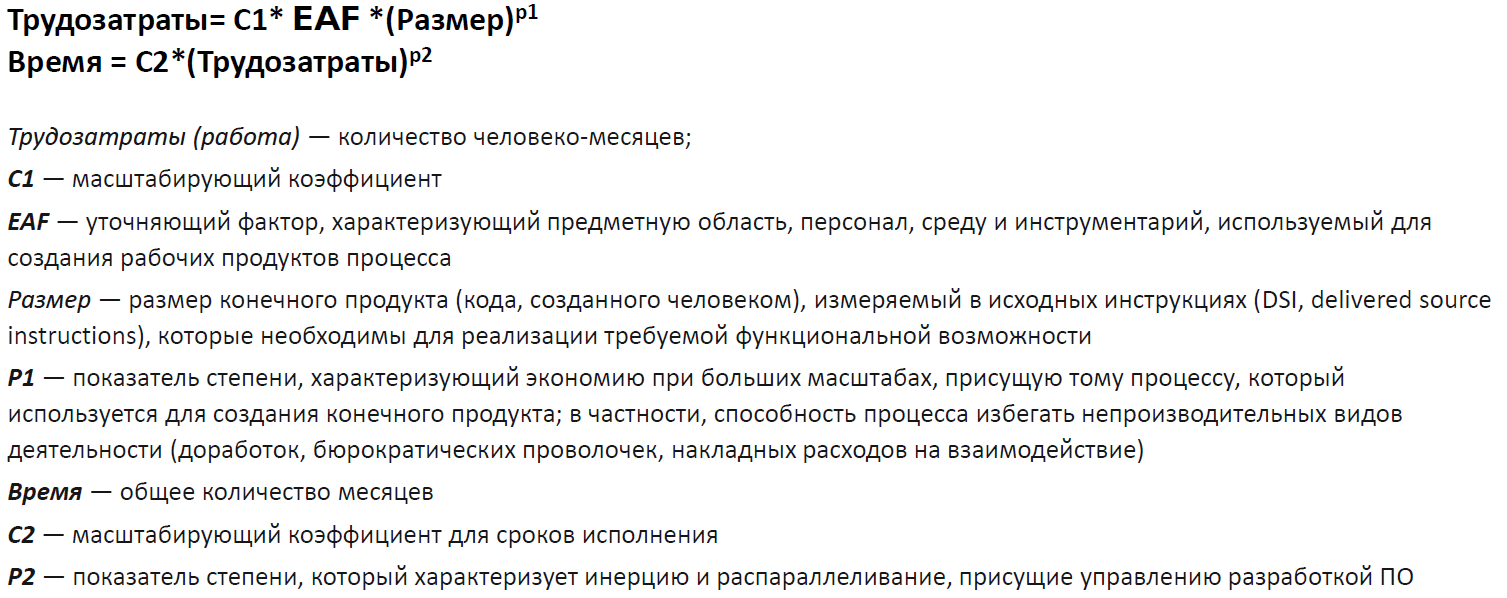
\includegraphics[width=1\linewidth]{inc/img/0.png}
	\caption{Модель оценки стоимости СОСОМО}
	\label{p0}
\end{figure}

Коэффициенты C1,C2, P1,P2 зависят от режима проекта (рис. \ref{p1}-\ref{p2}):
\begin{figure}[!h]
	\centering
	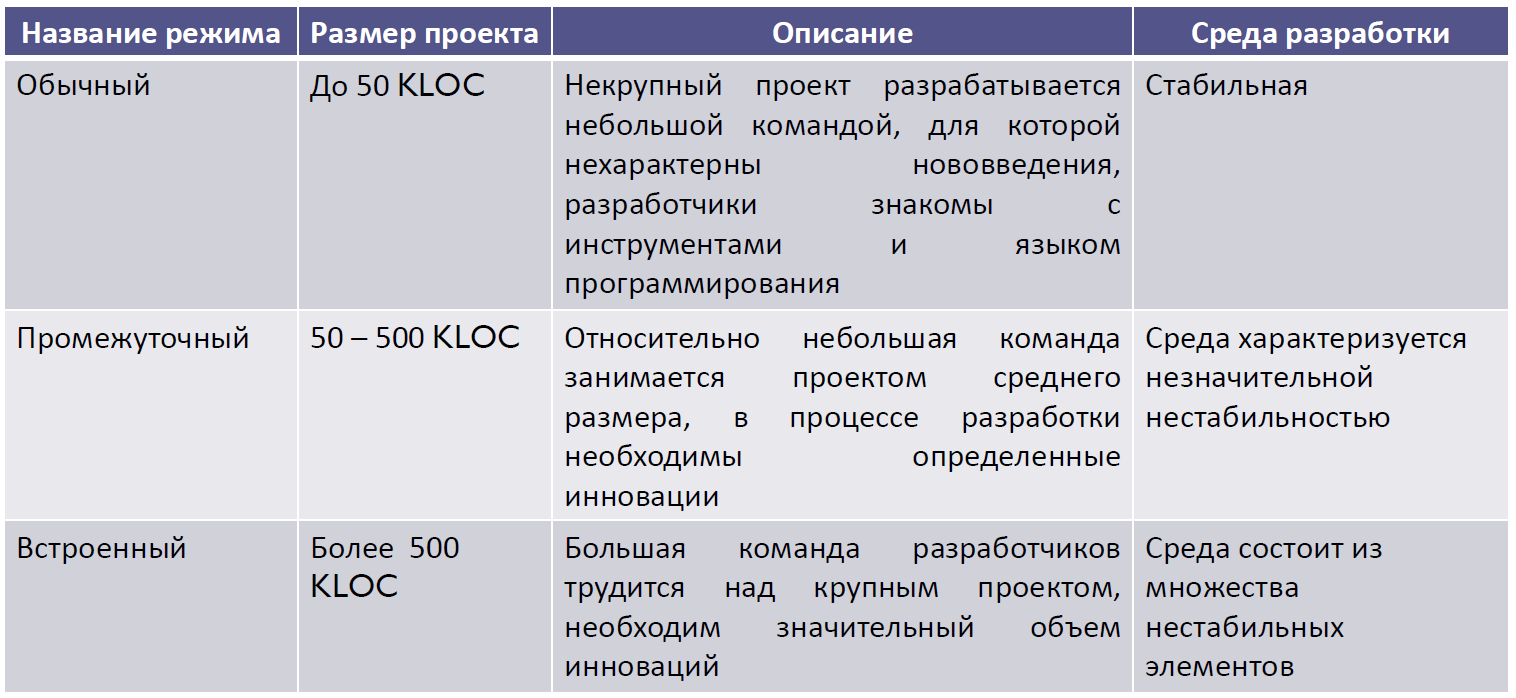
\includegraphics[width=1\linewidth]{inc/img/1.png}
	\caption{Режимы модели СОСОМО}
	\label{p1}
\end{figure}

\begin{figure}[!h]
	\centering
	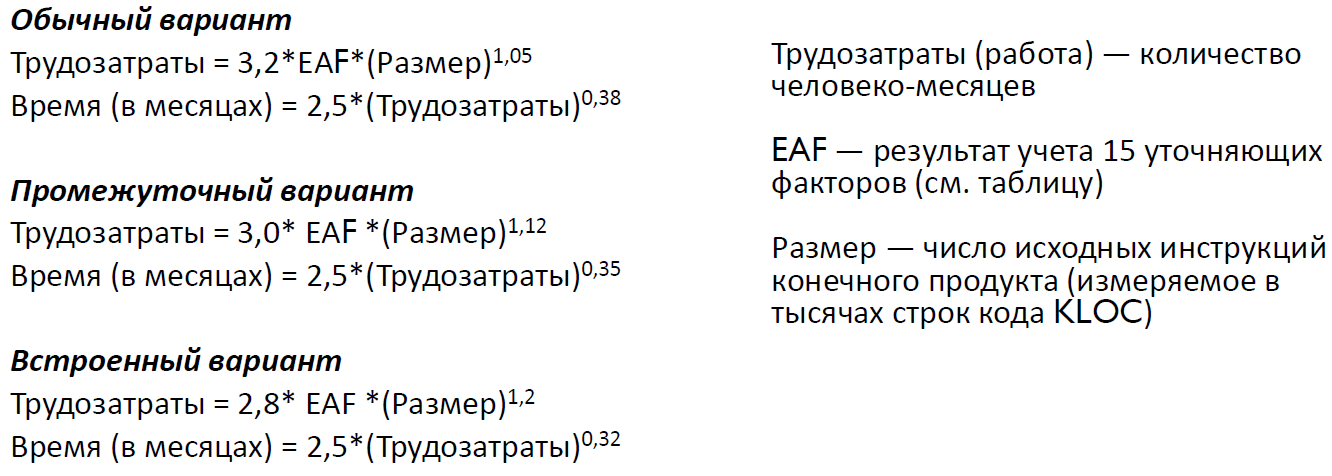
\includegraphics[width=1\linewidth]{inc/img/2.png}
	\caption{Формулы для оценки основных работ и сроков}
	\label{p2}
\end{figure}

\section*{Задание 1}
Исследовать степень влияния различных драйверов затрат на трудоемкость (РМ) и время разработки (ТМ) для модели COCOMO. Для это проанализировать, как меняется трудоемкость и время выполнения проекта при различных уровнях автоматизации среды (драйверы MODP – использование современных методов и TOOL – использование программных инструментов) и разном уровне способностей ключевых членов команды (драйверы ACAP – способности аналитика, PCAP – способности программиста). Взять за основу любой из типов проекта (обычный, встроенный или промежуточный) и при фиксированном значении размера программного кода (SIZE) получить значения PM и ТМ, изменяя значения указанных драйверов от очень низких до очень высоких. Результаты исследований оформить графически и сделать соответствующие выводы. При необходимости сократить срок выполнения проекта, что повлияет больше: способности персонала или параметры среды? При высоком уровне автоматизации (оба драйвера MODP и TOOL высокие) что окажет большее влияние на трудоемкость и время выполнения: высокая сложность продукта (параметр CPLX) или высокие ограничения на требуемые сроки разработки (параметр SCED)?

Необходимо провести сравнительный анализ атрибутов:
\begin{itemize}
	\item ACAP - способности аналитика;
	\item PCAP - способности программиста;
	\item MODP - использование современных методов;
	\item TOOL - использование программных инструментов;
	\item CPLX - сложность продукта;
	\item SCED - требуемые сроки разработки.
\end{itemize}

Все замеры будут проводиться при KLOC = 55, при промежуточном режиме работы, значения всех атрибутов, за
исключением исследуемых, будут принимать значение «номинальный».

\begin{figure}[!h]
	\centering
	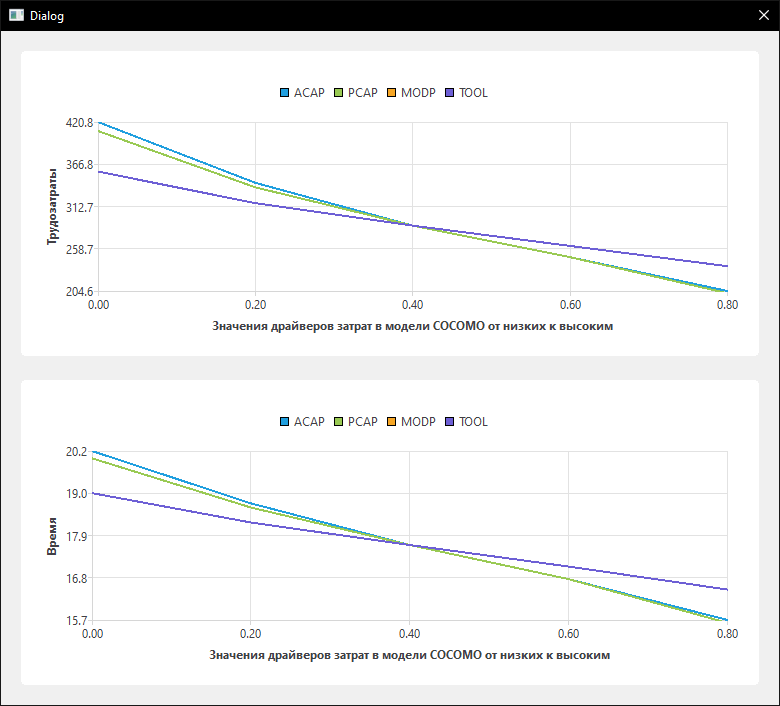
\includegraphics[width=1\linewidth]{inc/img/3.png}
	\caption{Результаты задания 1}
	\label{p3}
\end{figure}

Проанализировав информацию, которую отображают графики можно
сделать вывод, что с ростом параметров, уменьшаются трудозатраты, что в свою
очередь влияет на время реализации проекта.

При необходимости сократить срок выполнения проекта большее влияние окажут способности аналитиков и программистов.

При высоком уровне автоматизации, высокая сложность продукта (CPLX = 1,15) окажет большее влияние на трудоемкость, чем высокие ограничения на требуемые сроки разработки (SCED = 1,04).

\section*{Задание 2}
При разработке программного проекта его размер оценивается примерно в 55 KLOC. Этот проект будет представлять собой Web-систему, снабженную устойчивой серверной базой данных. Предполагается применение промежуточного варианта. Проект предполагает создание продукта средней сложности с номинальными требованиями по надежности, но с расширенной базой данных. Квалификация персонала средняя. Однако способности аналитика высокие. Оценить параметры проекта.

Занесем настройки проекта и проанализируем результаты (рис. \ref{p5}):
\begin{figure}[!h]
	\centering
	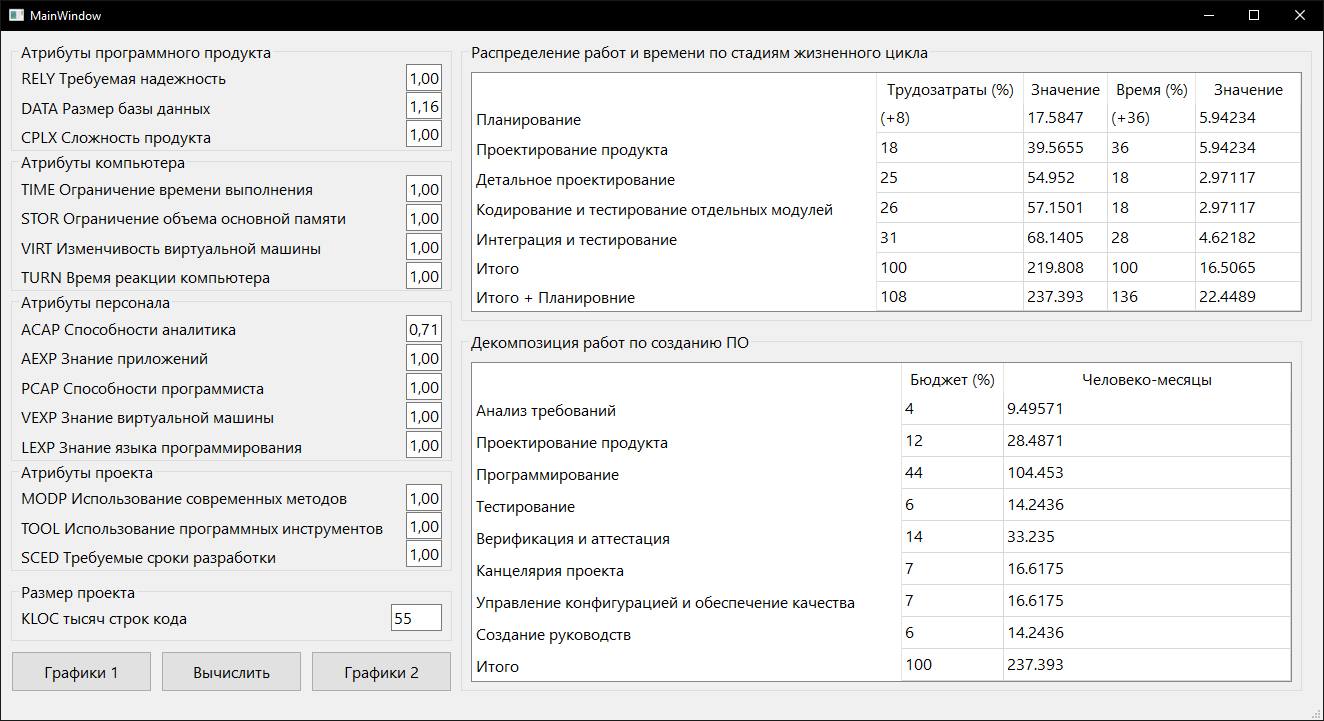
\includegraphics[width=1\linewidth]{inc/img/4.png}
	\caption{Результаты задания 2}
	\label{p4}
\end{figure}

Трудозатраты (с учетом планирования) = 237.393

Время (с учетом планирования) = 22.4489

\newpage 
\begin{figure}[!h]
	\centering
	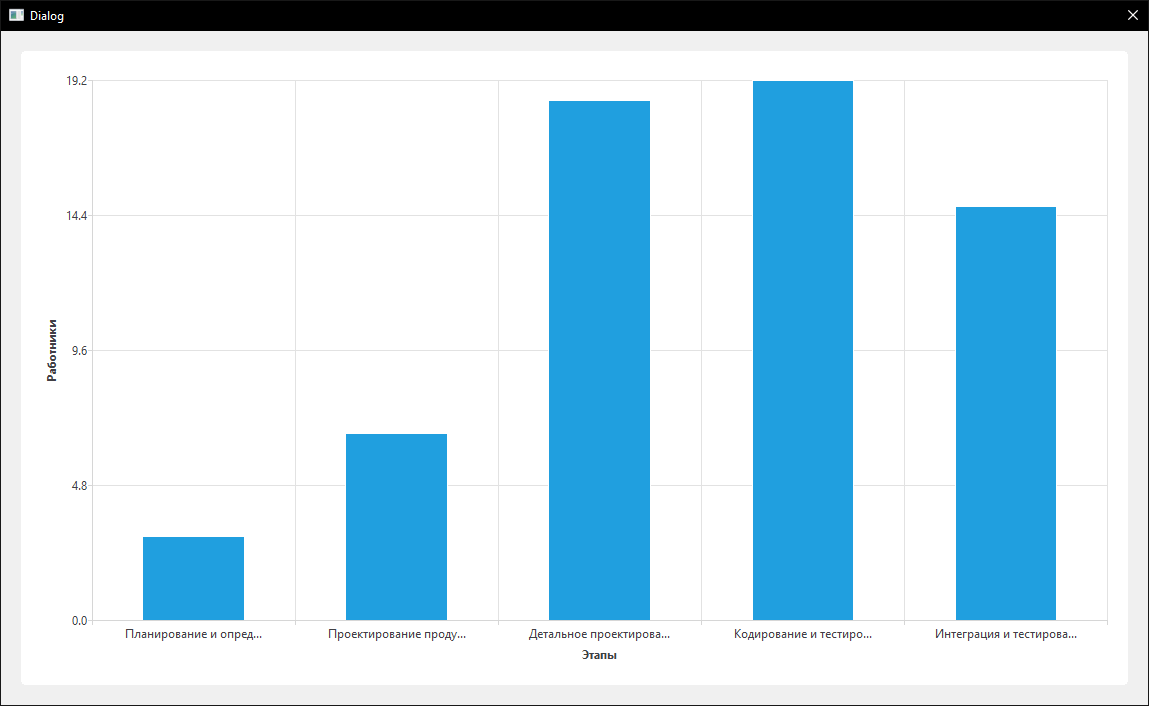
\includegraphics[width=1\linewidth]{inc/img/5.png}
	\caption{Результаты задания 2}
	\label{p5}
\end{figure}

На диаграмме привлечение сотрудников видно, что 3 и 4й этапы (детальное
проектирование; кодирование и тестирование) требует наибольшее количество
сотрудников.

\section*{Выводы}
В результате выполнения лабораторной работы был разработан
программный инструмент для оценки проекта по методике COCOMO. Были
изучены существующие методики предварительной оценки параметров
программного проекта, а также проведена практическая оценка затрат проекта.

По результатам применения методики оценки COCOMO можно
заключить, что она пригодна для общей предварительной оценки всего проекта
и позволяет получить приблизительные значения трудозатрат и времени на
реализацию проекта, разделенные на стадии его жизненного цикла. Однако для
постоянного отслеживания состояния проекта рекомендуется использовать
другие методики управления проектами с использованием различных
программных средств, которые позволяют актуализировать данные проекта в
реальном времени.